В данной задаче рассматривалось распределение фильмов по возрастным ограничениям и годам. Рассматривались только фильмы с наличием возрастного ограничения. Всего имеется пять разных возрастных ограничений - 0, 6, 12, 16 и 18 лет. Из Рис.~\ref{fig:films_number_by_age_limit_calculation} видно, что до 1960-х годов фильмов с возрастным ограничением почти не было. Далее до 1990-х годов фильмов 16+ было существенно больше, чем всех остальных, а начиная с 1990-х годов стало больше фильмов 18+. В последнее время фильмов 16+ и 18+ стало примерно одинаково, фильмов 12+ в 2 раза меньше, фильмов 6+ в 4 раза меньше и фильмов 0+ в 8 раз меньше.

\begin{figure}[ht!]
	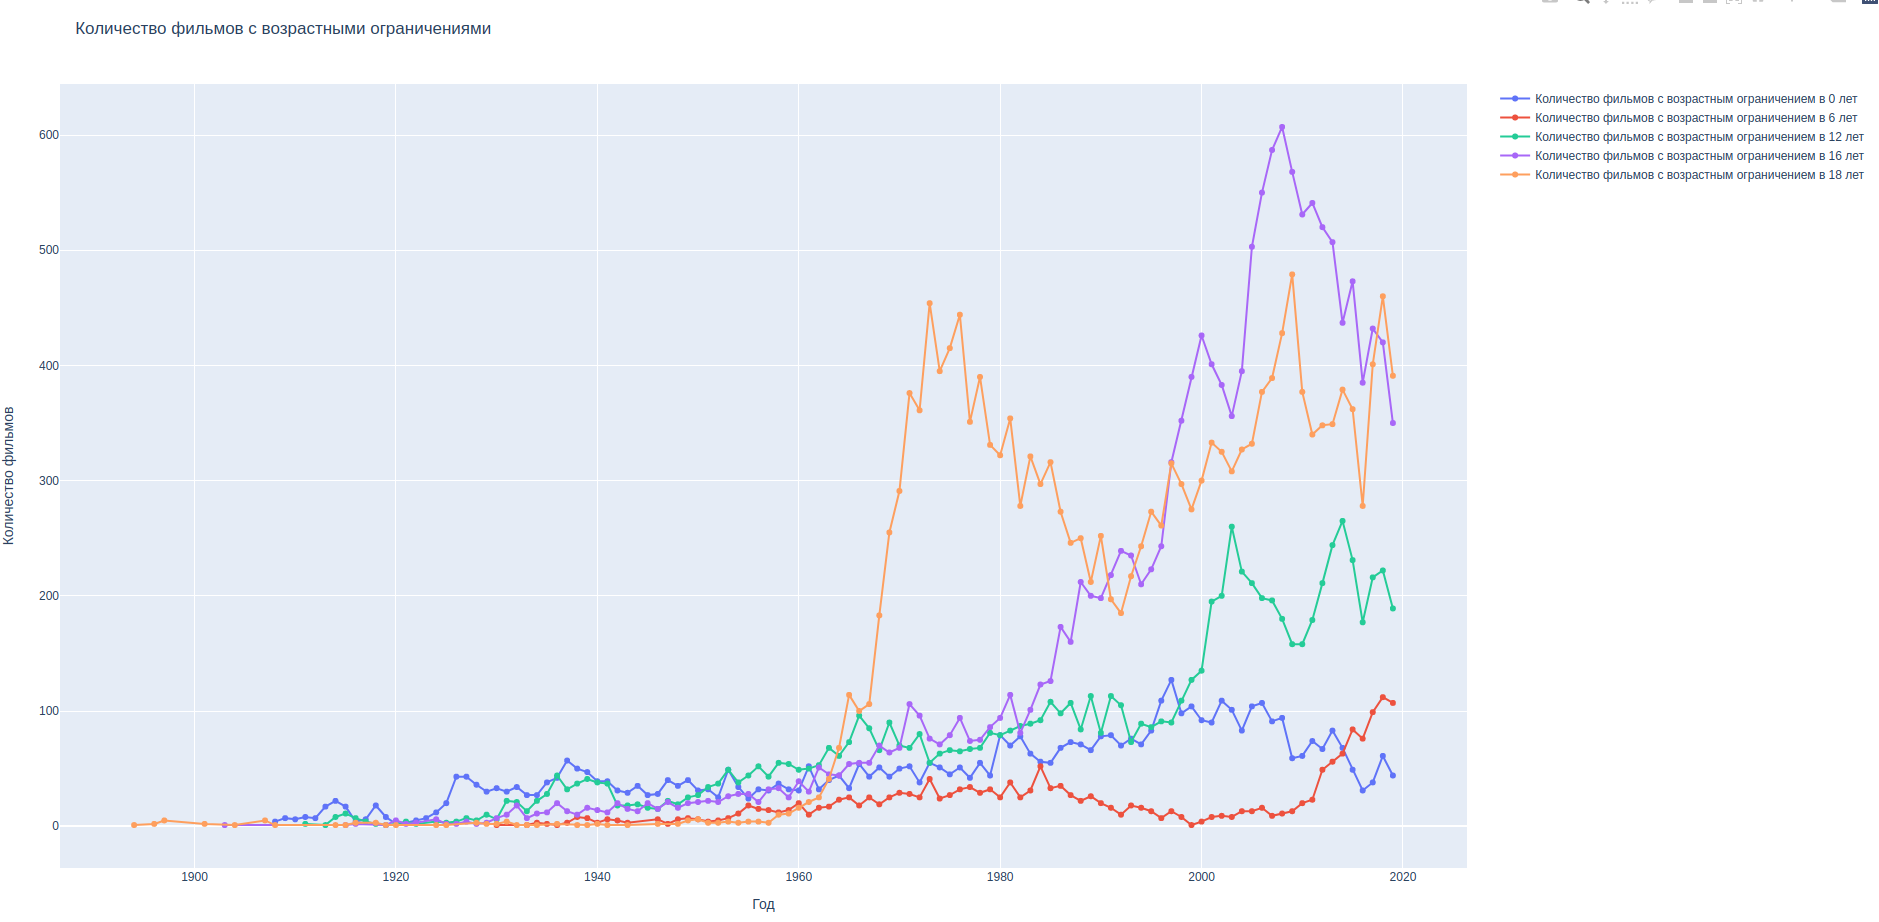
\includegraphics[width=\linewidth]{../report/images/years_restrict/1}
	\caption{Распределение фильмов по возрастным ограничениям и годам.}
	\label{fig:films_number_by_age_limit_calculation}
\end{figure}



